\documentclass[12pt]{article}

\begin{document}
\title{A RESEARCH ON DISTRIBUTION OF STUDENTS OF DIFFERENTS COURSES }
\author{MUGABI SAMUEL 15/U/7793/PS}
\date{May, 21, 2017}
\maketitle

\section{OUTLINE}
Problem statement		Scope		Methods used to collect data	Materials used 	Analysis of data
\section{PROBLEM STATEMENT}
To find out  the distribution of students of different coarses around campus hostels.

\subsection{SCOPE}
In this research, hostels and homes around campus and halls in campus are covered. 

\section{METHODS USED TO COLLECT DATA}
\textbf{Interviews;}
I interviewed different students asking them the courses they take and where they stay.
\textbf{ODK collect}
ODK collect was used to record information from the interviews, take a snap of the student, take the GPS coordinates and record date and time of collection of the data. 

\section{MATERIALS USED}
\textbf{A personal computer}
This was used to access the internet for software and uploading work to github
\textbf{An smart phone}
ODK collect was installed on my android device for collecting data
\textbf{Open Data Kit}
A form designed using ODK build, through ODK collect, was used to record information from the interviews, take a snap of the student, take the GPS coordinates and record date and time of collection of the data. Data collected was later sent to an aggregate server at http://trialprojected.appspot.com
\textbf{Google AppEngine platform}
This was used to build the aggregate server

\section{ANALYSIS OF DATA}
pie chart is found in the github folder
From the pie chart data collected shows that;
 55 percent of the students reside in Nakiyingi hostel.
15 percent of the students reside home.
10 percent of the students reside in Olympia hostel.
5 percent of the students reside in Nankulabye.
5 percent of the students reside in Mish hostel.
5 percent of the students reside in Livingstone hall.
Courses
The bar graph shows that most of the students are doing computer science followed by business statistics
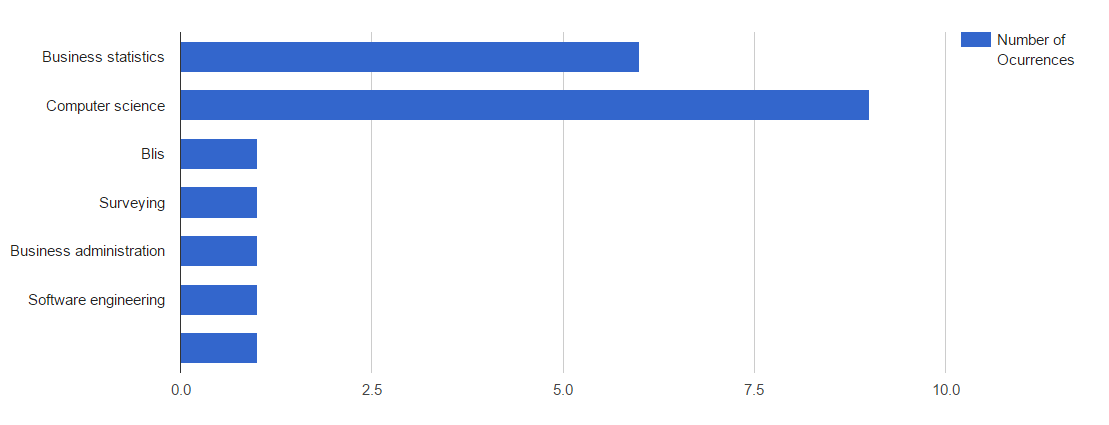
\includegraphics[]{G:/bar graph showing number of students and their courses.png}




\end{document}
